\documentclass[smaller,leqno]{beamer}

\setbeamersize{text margin left=3.5mm, text margin right=3.5mm}
\setbeamerfont{itemize/enumerate subbody}{size=\normalsize}
\setbeamertemplate{navigation symbols}{}
\setbeamertemplate{footline}[frame number]
\setbeamertemplate{blocks}[rounded]
\setbeamercolor{block title}{bg=black!30}
\setbeamercolor{block body}{bg=black!20}

\usepackage[utf8]{inputenc}
\usepackage[T1]{fontenc}
\usepackage{sansmath}
\usepackage{helvet}
\usepackage{inconsolata}
\usepackage{stmaryrd}

\usepackage{setspace}
\usepackage{listings}
\lstset{columns=flexible,basicstyle=\ttfamily,keywordstyle=\color{blue}}
\lstset{
	language=Haskell,
	deletekeywords={Monad,Functor},
	emph={pure},
	emphstyle=\color{red},
	literate={<*>}{{\color{red}<*>}}3,
	keepspaces}

\usepackage{tikz}
\usetikzlibrary{positioning}

\newenvironment{reference}{\begingroup\scriptsize\singlespacing\color{gray}}{\par\endgroup}
\DeclareMathOperator{\pure}{pure}
\newcommand{\ap}{\diamond}
\newcommand{\lba}[1]{\llbracket #1\rrbracket}

\title{Applicative Functors in Isabelle/HOL}
\author{Joshua Schneider \\ \texttt{joshuas@student.ethz.ch}}
\date{December 8, 2015}

\begin{document}

\begin{frame}
\titlepage
\end{frame}

\section{Introduction} %%%%%%%%%%%%%%%%%%%%%%%%%%%%%%%%%%%%%%%%%%%%%%%%%%%%%%%%

\begin{frame}[fragile]
\frametitle{Introduction: Tree Labels}

\begin{lstlisting}
data Tree a = Leaf a | Node (Tree a) (Tree a)
\end{lstlisting}

\begin{center}\begin{tikzpicture}[
	inner/.style={fill, circle, inner sep=2},
	leaf/.style={draw, circle, minimum size=20},
	subst/.style={dotted, thick},
	sibling distance=60, level distance=30, on grid]
\node[inner] {}
	child { node[leaf] (n1) {\alt<3>{1}{c}} }
	child { node[inner] {}
		child { node[leaf] (n2) {\alt<3>{2}{a}} }
		child { node[leaf] (n3) {\alt<3>{3}{b}} }
	};
\uncover<2>{
\node[below=2 of n1] {1} edge[subst] (n1);
\node[below=1 of n2] {2} edge[subst] (n2);
\node[below=1 of n3] {3} edge[subst] (n3);
}
\end{tikzpicture}\end{center}

\vspace{\fill}
\begin{reference}
Inspired by
G.\ Hutton and D.\ Fulger, ``Reasoning About Effects: Seeing the Wood Through the Trees.''
in \emph{Proceedings of the Symposium on Trends in Functional Programming}, (Nijmegen, The Netherlands, 2008).
\end{reference}
\end{frame}

\begin{frame}[fragile]
\frametitle{Composing Stateful Computations}

\begin{columns}[t,onlytextwidth]
\column{0.4\textwidth}
Standard solution: \\state monad
\vspace{5mm}
\begin{lstlisting}
fresh = do
  x <- get
  put (x + 1)
  return x
\end{lstlisting}

\begin{uncoverenv}<2->\begin{lstlisting}
numberTree (Leaf _)   = do
  x <- fresh
  return (Leaf x)
numberTree (Node l r) = do
  l' <- numberTree l
  r' <- numberTree r
  return (Node l' r')
\end{lstlisting}\end{uncoverenv}

\column<3->{0.55\textwidth}
Applicative style
\vspace{5mm}
\begin{lstlisting}
class Applicative m => Monad m where
  ...
class Functor f => Applicative f where
  pure  :: a -> f a
  (<*>) :: f (a -> b) -> f a -> f b
\end{lstlisting}

\begin{uncoverenv}<4>\begin{lstlisting}
numberTree (Leaf _)   =
  pure Leaf <*> fresh

numberTree (Node l r) =
  pure Node <*>
    numberTree l <*> numberTree r
\end{lstlisting}\end{uncoverenv}
\end{columns}

\vspace{\fill}
\begin{uncoverenv}<3->\begin{reference}
C.\ McBride and R.\ Paterson, ``Applicative Programming with Effects.''
\emph{Journal of Functional Programming, 18}~(1). 2008, 1--13.
\end{reference}\end{uncoverenv}
\end{frame}

\begin{frame}[fragile]
\frametitle{Renaming Trees and Lists}
%\begin{center}\begin{tikzpicture}[
%	inner/.style={fill, circle, inner sep=2},
%	leaf/.style={draw, circle, minimum size=20},
%	subst/.style={dotted, thick},
%	every node/.style={transform shape},
%	sibling distance=60, level distance=30, on grid, scale=0.7]
%\node[inner] (a) {}
%	child { node[leaf] (a1) {c} }
%	child { node[inner] {}
%		child { node[leaf] (a2) {a} }
%		child { node[leaf] (a3) {b} }
%	};
%\node[inner, below=3 of a] (b) {}
%	child { node[leaf] (b1) {1} }
%	child { node[inner] {}
%		child { node[leaf] (b2) {2} }
%		child { node[leaf] (b3) {3} }
%	};
%\node[left=2 of b1] {\texttt{numberTree}};
%\node[leaf, below=2.5 of b1] (x1) {1};
%\node[leaf, below=1.5 of b2] (x2) {2} edge [<-] (x1);
%\node[leaf, below=1.5 of b3] (x3) {3} edge [<-] (x2);
%\node[left=2 of x1] {\texttt{labels}};
%
%\node[inner, right=7 of a] (c) {}
%	child { node[leaf] (c1) {c} }
%	child { node[inner] {}
%		child { node[leaf] (c2) {a} }
%		child { node[leaf] (c3) {b} }
%	};
%\node[leaf, below=3 of c1] (d1) {c};
%\node[leaf, below=2 of c2] (d2) {a} edge [<-] (d1);
%\node[leaf, below=2 of c3] (d3) {b} edge [<-] (d2);
%\node[leaf, below=2.5 of d1] (y1) {1};
%\node[leaf, below=2.5 of d2] (y2) {2} edge [<-] (y1);
%\node[leaf, below=2.5 of d3] (y3) {3} edge [<-] (y2);
%
%\node[left=2 of d1] {$=$};
%\end{tikzpicture}\end{center}
%
%\pause
\begin{lstlisting}
labels (Leaf x)   = [x]
labels (Node l r) = labels l ++ labels r
\end{lstlisting}

\begin{uncoverenv}<2->\begin{lstlisting}
numberList []     = pure []
numberList (x:xs) = pure (:) <*> fresh <*> numberList xs

numberTree (Leaf _)   = pure Leaf <*> fresh
numberTree (Node l r) = pure Node <*> numberTree l <*> numberTree r
\end{lstlisting}\end{uncoverenv}

\begin{uncoverenv}<3>
\begin{block}{Proposition}\begin{lstlisting}
pure labels <*> numberTree t = numberList (labels t)
\end{lstlisting}\end{block}

Proof by induction on $t$. Leaf case:
\begin{lstlisting}
pure labels <*> (pure Leaf <*> fresh) = pure (:) <*> fresh <*> pure []
\end{lstlisting}
Compare with
\begin{lstlisting}
     labels     (     Leaf       x  ) =      (:)       x            []
\end{lstlisting}
\end{uncoverenv}
\end{frame}

\section{Proving Lifted Equations} %%%%%%%%%%%%%%%%%%%%%%%%%%%%%%%%%%%%%%%%%%%%

\begin{frame}[fragile]
\frametitle{A Proof Method for Isabelle}

\begin{block}{Project Goal}
Implement a proof method for Isabelle/HOL which lifts equations to
applicative functors.
\[ \text{base equation} \Longrightarrow \text{lifted equation} \]
\end{block}

\pause\vspace{3mm}
\begin{itemize}
\item Proof method: User interface for goal state transformation
\vspace{3mm}
\item Applicative functor or \emph{idiom} given by \begin{itemize}
	\item type constructor
	\item constants $\pure$, $\ap$ (\lstinline|<*>| in Haskell)
	\item proofs of applicative functor laws
\end{itemize}
\pause\vspace{3mm}
\item Lifting an equation ($x$ is a variable): $[\,] \mathbin{@} x = x$
\[ \begin{array}{rrcrcrcc}
\text{base equation:}\quad & \mathit{append} && [\,] && x &= & x \\[1ex]
\Longrightarrow\quad & \pure{\>\mathit{append}} &\ap& \pure{[\,]} &\ap& x & = & x
\end{array} \]
\end{itemize}
\end{frame}

\begin{frame}
\frametitle{Overview of Operation}

\begin{alignat*}{2}
\intertext{Input: Lifted equation}
&& e_1 &= e_2 \\
\intertext{Transform into \emph{canonical forms}}
&\Longleftarrow\quad & \pure f \ap x_1 \ap \dots \ap x_n &= \pure g \ap x_1 \ap \dots x_n
\action<2->{\intertext{Reduce by congruence}}
\action<2->{&\Longleftarrow\quad & f &= g}
\action<2->{\intertext{Extensionality}}
\action<2->{&\Longleftarrow\quad & \forall y_1 \dots y_n. \quad f y_1 \dots y_n &= g y_1 \dots y_n}
\end{alignat*}
\end{frame}

\begin{frame}
\frametitle{Hinze's Lemmas}

\begin{lemma}[Normal Form]
Let $e$ be an idiomatic term with variables $x_1,\dots,x_n$, from left to right.
There exists $f$ such that
\[ e = \pure f \ap x_1 \ap \dots \ap x_n. \]
\end{lemma}

Can lift equations
\begin{enumerate}
\item where both sides have the same list of variables, and
\item no variable is repeated.
\end{enumerate}

\begin{uncoverenv}<2->
\vspace{5mm}
\begin{lemma}[Lifting Lemma, modified]
Let $e'$ be the lifted term of $e$, with variables $x_1,\dots,x_n$.
If the idiom satisfies additional properties, then
\[ e' = \pure e \ap x_1 \ap \dots \ap x_n.  \]
\end{lemma}

Lifts any equation, but not to all applicative functors.
\end{uncoverenv}

\vspace{\fill}
\begin{reference}
R.\ Hinze, ``Lifting Operators and Laws.'' 2010. Retrieved June 6, 2015,
\url{http://www.cs.ox.ac.uk/ralf.hinze/Lifting.pdf}
\end{reference}
\end{frame}

\section{Combinators and Bracket Abstraction} %%%%%%%%%%%%%%%%%%%%%%%%%%%%%%%%%

\begin{frame}
\frametitle{Combinatory Logic}

\begin{itemize}
\item Eliminate variables from terms, introduce combinator constants
\item BCKW system is equivalent to lambda calculus
\begin{align*}
\mathbf{B} g f x &= g (f x) \\
\mathbf{C} f x y &= f y x \\
\mathbf{K} x y &= x \\
\mathbf{W} f x &= f x x
\end{align*}
\begin{uncoverenv}<2->
\item If not all combinators are available, not all terms can be represented
\item Conversion by \emph{bracket abstraction} algorithms
\end{uncoverenv}
\end{itemize}

\vspace{\fill}
\begin{reference}
H.\ B.\ Curry et.\ al., \emph{Combinatory Logic,} vol. 1.
North-Holland, Amsterdam, 1968.
\end{reference}
\end{frame}

\begin{frame}
\frametitle{Fancier Idioms}

\begin{itemize}
\item Some idioms satisfy additional laws, one or more of
\begin{alignat*}{2}
\pure \mathbf{C} \ap f \ap x \ap y &= f \ap y \ap x \tag{c} &\hspace{6em} \mathbf{C} f x y &= f y x \\
\pure \mathbf{K} \ap x \ap y &= x \tag{k} & \mathbf{K} x y &= x \\
\pure \mathbf{W} \ap f \ap x &= f \ap x \ap x \tag{w} & \mathbf{W} f x &= f x x
\end{alignat*}
\item Hinze's Lifting Lemma requires all three laws
\item Examples

\vspace{1mm}
\begin{tabular}{lccc}
 & (c) & (w) & (k) \\\hline
state monad & -- & -- & -- \\
set (application via Cartesian product) & (c) & -- & -- \\
sum type, e.g. \lstinline|Either| & -- & (w) & -- \\
option/\lstinline|Maybe| & (c) & (w) & -- \\
environment functor, streams & (c) & (w) & (k)
\end{tabular}
\end{itemize}
\end{frame}

\begin{frame}
\frametitle{Lifting Bracket Abstraction}

\begin{itemize}
\item Assume an applicative functors satisfies (c)
\begin{alignat*}{2}
\quad& \lambda x y.\> x (f y) & \quad& x \ap (\pure f \ap y) \\
=\quad& \mathbf{C B} f & \quad\qquad=\quad& \pure \mathbf{C} \ap \pure \mathbf{B} \ap \pure f \ap x \ap y \\
& & \qquad=\quad& \pure{(\mathbf{C B} f)} \ap x \ap y \\
& & \qquad=\quad& \pure{(\lambda x y.\> x (f y))} \ap x \ap y
\end{alignat*}

\item We obtain a canonical form if the base term is representable
\pause\item Variable order for idiomatic terms? Remember
\[ \pure f \ap x_1 \ap \dots \ap x_n = \pure g \ap x_1 \ap \dots x_n \]
\end{itemize}
\end{frame}

\section{Usage and Conclusion} %%%%%%%%%%%%%%%%%%%%%%%%%%%%%%%%%%%%%%%%%%%%%%%%%

\begin{frame}
\frametitle{Usage (1)}
\begin{center}
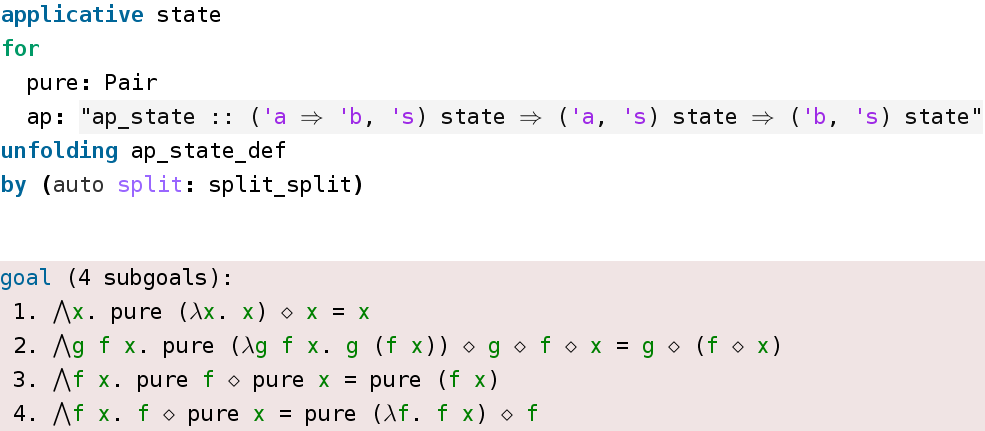
\includegraphics[width=\textwidth]{screenshot1.png}
\end{center}
\end{frame}

\begin{frame}
\frametitle{Usage (2)}
\begin{center}
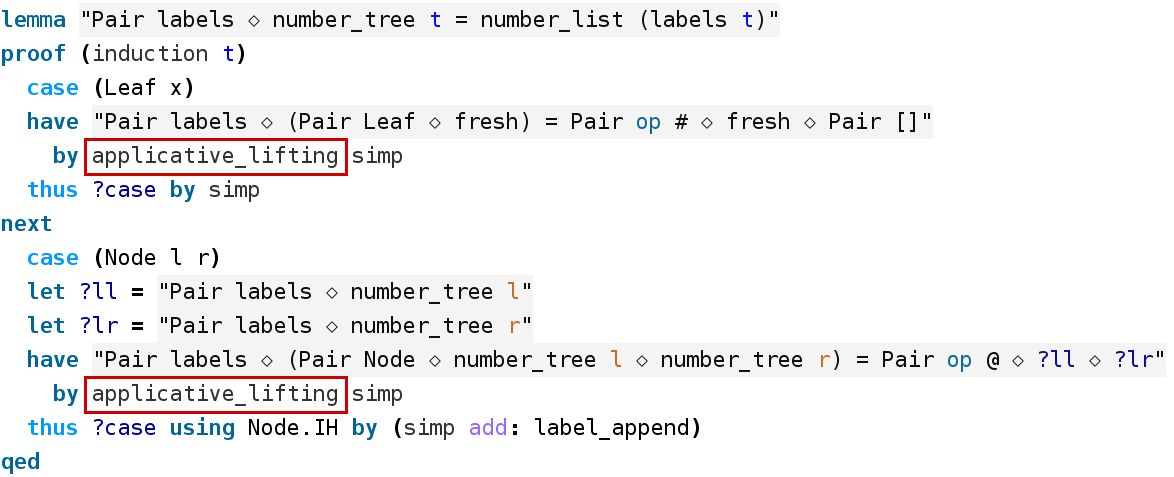
\includegraphics[width=\textwidth]{screenshot2.png}
\end{center}
\end{frame}

\begin{frame}
\frametitle{Conclusion}
\begin{itemize}
\item Implemented applicative lifting in Isabelle/HOL
\item Extended Hinze's results with bracket abstraction
\item Use case: Algebra lifted to streams and infinite trees
\end{itemize}

\vspace{10mm}
\begin{center}\large Questions?\end{center}
\end{frame}

\appendix %%%%%%%%%%%%%%%%%%%%%%%%%%%%%%%%%%%%%%%%%%%%%%%%%%%%%%%%%%%%%%%%%%%%%

\begin{frame}
\frametitle{Applicative Functor Laws}

\begin{align*}
	\tag{identity} \pure{\mathbf{I}} \ap u &= u \\[1ex]
	\tag{composition} \pure{\mathbf{B}} \ap u \ap v \ap w &= u \ap (v \ap w) \\[1ex]
	\tag{homomorphism} \pure{f} \ap \pure x &= \pure{(f x)} \\[1ex]
	\tag{interchange} u \ap \pure{x} &= \pure{(\lambda f.\> f x)} \ap u
\end{align*}
\end{frame}

\begin{frame}
\frametitle{Bracket Abstraction Rules}

\begin{alignat*}{2}
	\tag{$i$} [x]x &= \mathbf{I}, && \\
	\tag{$k$} [x]t &= \mathbf{K} t &&\qquad\text{if $x$ not free in $t$}, \\
	\tag{$\eta$} [x]tx &= t &&\qquad\text{if $x$ not free in $t$}, \\
	\tag{$b$} [x]st &= \mathbf{B}s([x]t) &&\qquad\text{if $x$ not free in $s$}, \\
	\tag{$c$} [x]st &= \mathbf{C}([x]s)t &&\qquad\text{if $x$ not free in $t$}, \\
	\tag{$s$} [x]st &= \mathbf{S}([x]s)([x]t); && \\[2ex]
\intertext{Special rules for idioms:}
	\tag{$t$} [x]st &= \mathbf{T}t([x]s) &&\qquad\text{if $t$ contains no variables}, \\
	\tag{$w$} [x]st &= \mathbf{W}(\mathbf{B}(\mathbf{T}[x]t)(\mathbf{B}\mathbf{B}[x]s))
		&&\qquad\text{if $[x]t$ contains no variables}.
\end{alignat*}
\end{frame}

\begin{frame}
\frametitle{What are the Variables?}

\begin{itemize}
\item Remember that both canonical forms need the same variable lists:
\[ \pure f \ap x_1 \ap \dots \ap x_n = \pure g \ap x_1 \ap \dots x_n \]
\item Must be able to represent terms with available combinators
\item Instantiation:
\begin{alignat*}{2}
	& \forall x y. \; & \pure f \ap x \ap y &= \dots \\
	\Longrightarrow\quad & \forall z. \; & \pure f \ap z \ap z &= \dots
\end{alignat*}
What if we want to prove the latter, but can only represent the former?
\item Algorithm depends on available combinators, partially a heuristic
\end{itemize}
\end{frame}


\end{document}
